\section{Teori}

\subsection{Euler-Bernoulli}
Flere av oppgavene i denne rapporten omhandler Euler-Bernoulli-teoremet. Vi skal blandt annet bruke det til å regne ut bøyningen i et stupebrett, men vi skal også regne litt på den korrekte løsningen av likningen. Først litt generelt om temoremet; I følge Wikipedia er dette en grunnleggende metode for å regne ut hvor mye en bjelke av et gitt materiale bøyer seg under press. Metoden er oppkalt etter Jacob Bernoulli som gjorde de største oppdagelsene, det var derimot ikke før rundt 1750 at Leonhard Euler og Daniel Bernoulli kom opp med en komplett teori. Metoden ble ikke brukt i praksis på noen større prosjekter før byggingen av Eiffeltårnet i 1889, men har siden blitt en hjørnestein innen ingeniørkunsten.\footnote{\url{https://en.wikipedia.org/wiki/Euler-Bernoulli_beam_theory}, (14.04.2016)} Euler-Bernoulli-likningen som vi skal bruke i disse oppgavene er som følger:
\begin{quote}
\begin{equation}
EIy''''=f(x)
\end{equation}
\end{quote}

Den vertikale forskyvningen av en $L$ meter lang bjelke, oppfyller likningen når $0\leq x\leq L$. Likningen inneholder noen konstanter; $E$ er en materialkonstant kalt Youngmodulusen. $I$ er et arealmoment til bjelkens tverrsnitt normalt på lengderetningen. $I$ er konstant langs hele bjelken. Høyresiden av likningen, $f(x)$, er en kraft som virker på bjelken per lengde-enhet målt i Newton per meter. Kraften inkluderer vekten til bjelken. Dette har vi fra læreboken. Vi skal i denne oppgaven kun bruke konstanter som er oppgitt i læreboka.\footnote{Sauer, Timothy, (2012) Numerical Analysis second edition, side 102-.}

Dette teoremet passer bra til et stupebrett, da vi kan se på dette som en bjelke som blir bøyd på grunn av last. Lastene vi skal se på senere i denne oppgaven er først en sinusformet haug og deretter en person. Da må vi utvide formelen vår ved å legge til følgende funksjoner til kraft-delen av likningen:
\begin{quote}
\begin{equation}
s(x)=-pg\;sin\frac{\pi}{L}x
\end{equation}
\begin{equation}
s_2(x)=\begin{cases}
	-g\cdot{50/0.3kg/m} & ,L-0.3m\leq x\leq L\\
	0N/m & ,0m\leq x\leq L-0.3m
	\end{cases}
\end{equation}
\end{quote}
Vi legger til $s(x)$ for den sinusformede haugen og $s_2(x)$ for personen. 

\subsection{Taylors Teorem}
Taylors Teorem er en måte å estimere en gitt funksjon på ved hjelp av polynomer. Man kan se på Taylors formel som en generalisering av "Mean Value Theorem", som sier at dersom funksjonen f er kontinuerlig i et lukket intervall [a,b] og f er deriverbar i det åpne intervallet (a,b), et punkt c, a < c < b eksisterer slik at :
\begin{quote}
\begin{equation}
f'(c) = \frac{f(b) - f(a)}{b-a}
\end{equation}
\end{quote}
Mer bestemt, la f være en funksjon slik at f og dens første n-deriverte er kontinuerlig i [a,b]. Videre, la $f^{(n+1)}(x)$ eksistere for alle x i (a,b). Da eksisterer det et tall c i (a,b) slik at:
\begin{quote}
\begin{equation}
f(b) = f(a) + (b-a) \frac{f'(a)}{1!} + (b-a)^2 \frac{f''(a)}{2!} + .... + (b-a)^n \frac{f^{(n)}}{n!} + (b-a)^{(n+1)} \frac{f^{(n+1} (c)}{(n+1)!}
\end{equation}
\end{quote}
Formelen sier også at dersom b < a, så vil [a,b] og (a,b) blir byttet ut med [b,a] og (b,a) henholdsvis. Man kan også se at dersom vi bytter ut b med x, står vi igjen med Taylor's formelen. \\
En annen måte å skrive Taylor's formelen på er
\begin{quote}
\begin{equation}
\sum_{i=0}^n (x-a)î \frac{f''(a)}{i!} + (x-a)^{n+1} \frac{f^{(n+1)} (c) }{(n+1)!}
\end{equation}
\end{quote}
som også er kjent som n-te grad Taylor polynom (eller Taylor serie) med feil ledd.\\
For å visualisere dette kan vi ta for oss funksjonen $f(x) = sin(x)$. Ved å regne ut flere ledd i Taylor-rekken vil vi kunne skape en tilnærming av funksjonen. Desto flere ledd, desto mer nøyaktig tilnærming:

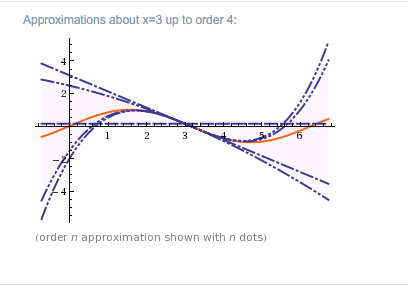
\includegraphics[width=\textwidth]{taylor_sinx}
Grafen er en taylors-rekke av f(x) = sin(x), der x=3. Studerer man de blå striplette linjene ser vi at de inneholder ulikt antall prikker. 1 prikk tilsvarer første deriverte, 2prikker tilsvarer andre deriverte osv. Ut i fra grafen ser man at dersom man har et høyere derivasjonsledd vil den blå linjen følge funksjonen mer og mer, og vi får en mer nøyaktig tilnærming av funksjonen. 


\subsection{Feil}
Når vi snakker om feil i nummerikk, snakker vi om nøyaktigheten i utregninger og hvor nært et riktig svar vi kan komme. Det er ofte snakk om hvor mange desimaler vi kan få riktig. Når vi regner med maskin vil vi grunnet avrundingen i flyttall få en maskin-feil epsilon som er $\epsilon_{mach} = 2^{-52}$. Dette gjør at det blir nesten umulig å regne med mer enn 16 desimalers nøyaktighet. Vi deler feil opp i bakover- og foroverfeil. Enkelt forklart er bakoverfeil feil med "inputen" til et problem, mens foroverfeil er feil med "outputen".

\subsubsection{Foroverfeil}
I vår oppgave jobber vi mest med matriselikninger og da har vi følgende definisjon på foroverfeil; Hvis vi for eksempel har matriselikningen $Ax = b$ med tilnærmet løsning $x_a$, får vi følgende definisjoner: 
\begin{quote}	
\begin{equation*}
\mbox{Foroverfeil} = ||x - x_a||_{\infty}
\end{equation*}
\begin{equation*}
\mbox{Relativ foroverfeil} = \frac{||x - x_a||_{\infty}}{||x||_{\infty}}
\end{equation*}
\end{quote}
Her vil $x$ og $x_a$ være vektorer/matriser, og det vi gjør er å ta uendelighetsnormen av dem. Å ta uendelighetsnormen betyr at vi finner den største absoluttverdien av alle radsummene i matrisen. I tilfeller hvor disse er vektorer blir det da største absoluttverdi i vektoren. På én oppgave finner vi også 1-normen av en matrise. Da finner vi summen av absoluttverdien av alle radsummene.

\subsubsection{Bakoverfeil}
Siden vi jobber mest med matriselikninger får vi følgende definisjon på bakoverfeil; Hvis vi for eksempel har matriselikningen $Ax = b$ med tilnærmet løsning $x_a$ og Residualet: $r = b - Ax_a$, får vi følgende definisjoner:
\begin{quote}	
\begin{equation*}
\mbox{Bakoverfeil} = ||r||_{\infty} = ||b-Ax_a||_{\infty}
\end{equation*}
\begin{equation*}
\mbox{Relativ bakoverfeil} = \frac{||r||_{\infty}}{||b||_{\infty}}
\end{equation*}
\end{quote}

\subsubsection{Feilforstørring}
Når vi regner med feil på denne måten kan det være greit å se hvordan bakoverfeil og foroverfeil påvirker hverandre. Feilforstørringsfaktoren er et slikt tall som viser sammenhengen mellom relativ foroverfeil og relativ bakoverfeil. Dette tallet regnes ut slik:
\begin{quote}
\begin{equation*}
\mbox{Feilforstørring} = \frac{\mbox{Relativ foroverfeil}}{\mbox{Relativ bakoverfeil}} = \frac{\frac{||x - x_a||_{\infty}}{||x||_{\infty}}}{\frac{||r||_{\infty}}{||b||_{\infty}}}
\end{equation*}
\end{quote}
 

 
 \subsection{Kondisjonstall}
Når vi snakker om kondisjonstallet til en funksjon f med et argument x måler vi omfanget av endringer i resultatet til f med liten endring i x. Vi bruker dette til å estimere hvor sensitiv en funksjon er til endringer eller feil i x, og størrelsen på feil som kan forekomme. I matrisesammenheng kan vi se på den lineære likningen Ax = b. Kondisjonstallet til A vil fortelle oss om hvor store endringene i b blir med små endringer i x. I MATLAB benytter vi oss av "cond(A)" for å finne kondisjonstallet. Denne metoden bygger på funksjonen:
 \
 \begin{equation}
 Cond(A) = ||A^{-1}|| \cdot ||A||
 \end{equation}
 
Dersom kondisjonstallet er 1 vil dette bety at en feil i x ikke vil kunne lage større skade enn feilen i seg selv. Så kort sagt er et lavt kondisjonstall bra, og et stort dårlig. 

USIKKER PÅ OM DETTE STEMMER, MÅ SJEKKES I MATLAB!!!:

Gitt matrisen A = $\begin{matrix}
 
	1 & 1/2\\
	1/2 & 1/3
	
\end{matrix}$
\\
og vektorene $b_1 = (2/3, 1)'$ og $b_2 = (2/3, 1)'$
\\Her skulle vi tro at $Ab_1$ og $Ab_2$ ville blitt ganske lik, men med å regne ut finner vi at:\\$x_1 = (0, 3)'$ og $x_2 = (1, 1)'$
\\Med dette ser vi at noen matriser er veldig sensitive til små endringer i inn-data.

\subsection{MATLAB}
For å løse de vanskeligste problemene i dette prosjektet, trenger vi hjelp fra et digitalt verktøy. Og vi bruker MatLab. MatLab, kort for Matrix Laboratory, er et omfattende matematikk-program utiklet av MathWorks. Siden programmet først ble utgitt i 1984 har det blitt et veldig populært program til bruk på utdanningsinstitusjoner. I 2004 hadde MatLab over 1 million registrerte lisenser på verdensbasis.
MatLab opererer med et eget script-språk basert på programmeringsspråket C, så det er veldig nyttig for oss dataingeniører. Med MatLab kan vi utføre matriseregning, behandle og plotte funksjoner, implementere algoritmer osv. Det at det opererer på et script-språk gjør også at vi kan skrive egne funksjoner for å løse problemer. Ved å skrive kode for å løse oppgavene er det lett for oss å vise fremgangsmåte i tillegg til riktig svar.
\subsubsection{Noen MATLAB-metoder vi bruker}
\textbf{hentKonstanter()}\\
Dette er en funksjon vi har laget selv. Denne bruker vi i flere av oppgavene våre. Det den gjør er å hente ut de konstantene vi har fått definert fra læreboka slik at vi slipper å definere nye variabler for hver gang de skal brukes. På denne måten har vi alltid variablene på plass når vi trenger dem.\\
\\
\textbf{repmat}\\
Brukes til å repetere n antall kopier av matrisen.\\
\\
\textbf{ones}\\
Lager en matrise av enere.\\
\\
\textbf{sparsediag}\\
Henter ut diagonale vektorer for ei sparsematrise. Hvor det ikke bare er 0’ere.\\
\\
\textbf{Zeros}\\
Lager en matrise av bare 0’ere.\\
\\
\textbf{abs(n)}\\
Tar absoluttverdien av n.\\
\\
\textbf{Table}\\
Brukes for å lage en tabell av input.\\
\\
\textbf{Plot}\\
Lager et vindu med for eksempel plot(X,Y) der dataen i Y korresponderer mot verdien i X.\\
\\
\textbf{Subplot}\\
Lager en matrise av plotfunksjonen med bestemt rad og rekke.

\subsection{Teori tilknyttet oppgaver}
\subsubsection{Oppgave 3}
Møtte på et problem tilknyttet oppgave 3 hvor vi fikk positive verdier for y. Etter lang leting viste det seg at i vår lagA- metode så hadde vi klart å skreve -157/17 kontra -156/17 som det egentlig skulle være. Var spennende å se at en så liten feil kunne resultere til så forskjellige verdier. 